\documentclass{beamer}
\mode<presentation> {
%\usetheme{Dresden}
\usetheme{CambridgeUS}
}
\newcommand{\subitem}{\par\qquad}
\usepackage{booktabs}

\usepackage{tikz}
\usepackage{subfigure}	
\usepackage[round]{natbib}   % omit 'round' option if you prefer square brackets
\DeclareMathOperator*{\argmin}{argmin}
\DeclareMathOperator*{\argmax}{argmax}

\usetikzlibrary{arrows,calc,positioning,decorations.pathreplacing} 
\tikzset{
	>=stealth',
	punkt/.style={
		circle,
		draw=black, thick,
		minimum height=2em,
		inner sep=0pt,
		text centered},
	pil/.style={
		->,
		thick,
		shorten <=2pt,
		shorten >=2pt,},
	cir/.style={
		rectangle,
		rounded corners,
		draw=black, thick,
		minimum width=1.5em,
		text centered},
	arr/.style={
		->,
		thick,
		shorten <=2pt,
		shorten >=2pt,},
	layer/.style={
		draw=black,
		fill=white,
		thick,
		rectangle,
		rounded corners,
		minimum width=1.5em,
		minimum height=12em
	},
	brace/.style={
		thick,
		decoration={
			brace,
			mirror,
			raise=2.5cm
		},
		decorate
	}
}

\newcommand{\drawlayer}[4]{
	\node[layer, draw=#4] (#1) at (#2,#3) {};
	\foreach \x in {-1.75, -1.25, -0.75, -0.25, 0.25, 0.75, 1.25, 1.75} \draw[thick, #4] (#2,\x+#3) circle (0.15);
}
\newcommand\irregularcircle[2]{
	\pgfextra {\pgfmathsetmacro\len{(#1)+rand*(#2)}}
	+(0:\len pt)
	\foreach \a in {10,20,...,350}{
		\pgfextra {\pgfmathsetmacro\len{(#1)+rand*(#2)}}
		-- +(\a:\len pt)
	} -- cycle
}

\newcommand{\independent}{\mbox{${}\perp\mkern-11mu\perp{}$}}
\newcommand{\notindependent}{\mbox{${}\not\!\perp\mkern-11mu\perp{}$}}
\newcommand{\iid}{\overset{\text{iid}}{\sim}}

%%%%%%%%%%%%%%%%%%%%%%%%%%%%%%%%%%%%%%%%%%%%%%%%%%%%%%%%%%%%%%%%%%%%%%%%%%
% PARENTHESES 
%%%%%%%%%%%%%%%%%%%%%%%%%%%%%%%%%%%%%%%%%%%%%%%%%%%%%%%%%%%%%%%%%%%%%%%%%%

\renewcommand{\dot}[2]{\langle {#1},\, {#2} \rangle}
\newcommand{\pa}[1]{\left( #1 \right)}
\newcommand{\pb}[1]{\left\{ #1 \right\}}
\newcommand{\pc}[1]{\left[ #1 \right]}
\newcommand{\pn}[1]{\left\| #1 \right\|}
\newcommand{\ps}[1]{\left| #1 \right|}
\newcommand{\ot}{\leftarrow}
\newcommand{\given}{\, | \,}

%%%%%%%%%%%%%%%%%%%%%%%%%%%%%%%%%%%%%%%%%%%%%%%%%%%%%%%%%%%%%%%%%%%%%%%%%%
% MATHCAL
%%%%%%%%%%%%%%%%%%%%%%%%%%%%%%%%%%%%%%%%%%%%%%%%%%%%%%%%%%%%%%%%%%%%%%%%%%

\newcommand{\D}{\mathcal{D}}
\renewcommand{\P}{\mathcal{P}}
\renewcommand{\Pr}{\mathbb{P}}
\renewcommand{\H}{\mathcal{H}}
\renewcommand{\L}{\mathcal{L}}
\newcommand{\Hk}{{\mathcal{H}_k}}
\newcommand{\F}{\mathcal{F}}
\newcommand{\X}{\mathcal{X}}
\newcommand{\Y}{\mathcal{Y}}
\newcommand{\Z}{\mathcal{Z}}
\newcommand{\N}{\mathcal{N}}
\newcommand{\Ex}{\mathcal{E}}
\newcommand{\Hyp}{\mathcal{H}}
\newcommand{\B}{\mathcal{B}}


%%%%%%%%%%%%%%%%%%%%%%%%%%%%%%%%%%%%%%%%%%%%%%%%%%%%%%%%%%%%%%%%%%%%%%%%%%
% MATHBB 
%%%%%%%%%%%%%%%%%%%%%%%%%%%%%%%%%%%%%%%%%%%%%%%%%%%%%%%%%%%%%%%%%%%%%%%%%%

\newcommand{\Pio}{\mathbb{P}}
\newcommand{\R}{\mathbb{R}}
\newcommand{\Rd}{\mathbb{R}^d}
\newcommand{\Rq}{\mathbb{R}^q}
\newcommand{\Rn}{\mathbb{R}^n}
\newcommand{\Rm}{\mathbb{R}^m}
\newcommand{\Rnd}{\mathbb{R}^{n \times d}}
\newcommand{\Rnm}{\mathbb{R}^{n \times m}}
\newcommand{\I}{\mathbb{I}}
\newcommand{\Pa}{\mathrm{Pa}}
\renewcommand{\d}{\mathrm{d}}
\newcommand{\sig}{\mathrm{sign}\circ\!}
\newcommand{\Rp}{R_{\varphi}}
\newcommand{\Rpn}{\hat{R}_{\varphi}}
\newcommand{\Rpnt}{\tilde{R}_{\varphi}}
\newcommand{\f}{f^*}
\newcommand{\fn}{\hat{f}_n}
\newcommand{\fnt}{\tilde{f}_n}
\newcommand{\fntm}{\tilde{f}^m_n}
\newcommand{\Mk}{\M_k}
\newcommand{\muP}{\mu_k(\P)}
\renewcommand{\d}{{\mathrm{d}}}
\newcommand{\Rad}{\mathrm{Rad}}
\newcommand{\M}{\mathscr{M}}
\newcommand{\head}[2]{\multicolumn{1}{>{\centering\arraybackslash}p{#1}}{\textbf{#2}}}
\renewcommand{\do}{do}
\title[KME for CI]{Kernel Mean Embedding for Causal Inference} 

\author[Behrad Moniri]{Behrad Moniri}

\institute[EE @ Sharif] 
{
Department of Electrical Engineering\\
Sharif University of Technology 
}

\titlegraphic{
\includegraphics[width=2cm]{logo.png}\hspace*{-8.75cm}~%
%	\includegraphics[width=2cm]{digilogo.png}
}
\newcommand{\bigCI}{\mathrel{\text{\scalebox{1.07}{$\perp\mkern-10mu\perp$}}}}

\begin{document}

\begin{frame}
\titlepage
\end{frame}

\begin{frame}
\centering
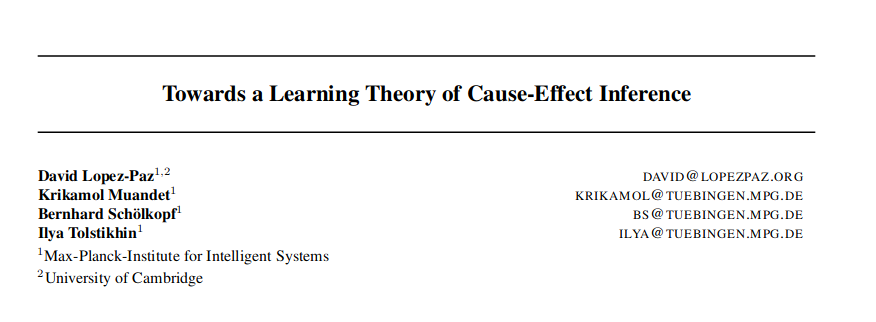
\includegraphics[scale=0.4]{lopez.png}

ICML - 2015
\end{frame}

\begin{frame}
\textbf{Main Contributions}: 
\begin{itemize}
	\item Learning causal relations directly from data.
	\item Distributional Learning Theory
	\item Improved Accuracy on MPI Cause Effect Pairs
\end{itemize}
\end{frame}

\subsection{Idea}
\begin{frame}
\frametitle{Main Idea of Paper}
\textbf{Causal inference can been seen as classification of probability distributions.} But it is unrealistic to assume have access to the whole distribution. All we know about the distribution is available through iid samples.

\vspace{1cm}
\tikzset{every picture/.style={line width=0.75pt}} %set default line width to 0.75pt        
\centering


\tikzset{every picture/.style={line width=0.75pt}} %set default line width to 0.75pt        

\begin{tikzpicture}[x=0.75pt,y=0.75pt,yscale=-1,xscale=1]
\draw   (261,98) -- (331,98) -- (331,138) -- (261,138) -- cycle ;
\draw    (218,118.67) -- (258,118.67) ;
\draw [shift={(260,118.67)}, rotate = 180] [color={rgb, 255:red, 0; green, 0; blue, 0 }  ][line width=0.75]    (10.93,-3.29) .. controls (6.95,-1.4) and (3.31,-0.3) .. (0,0) .. controls (3.31,0.3) and (6.95,1.4) .. (10.93,3.29)   ;
\draw    (332,118.67) -- (372,118.67) ;
\draw [shift={(374,118.67)}, rotate = 180] [color={rgb, 255:red, 0; green, 0; blue, 0 }  ][line width=0.75]    (10.93,-3.29) .. controls (6.95,-1.4) and (3.31,-0.3) .. (0,0) .. controls (3.31,0.3) and (6.95,1.4) .. (10.93,3.29)   ;


% Text Node
\draw (296,118) node  [align=left] {Classifier};
% Text Node
\draw (134,120) node  [align=left] {$\displaystyle \left\{\left( x^{j}_{i} \ ,\ y^{j}_{i}\right) \ \right\}_{j = 1}^{n_i} \sim  P_i^{n_i}$};
% Text Node
\draw (435,120) node  [align=left] {$\displaystyle x\rightarrow y\ \ or\ y\rightarrow \ x$};
\end{tikzpicture}
\end{frame}


\begin{frame}
\begin{center}
	\centering
	\includegraphics[scale=0.35]{figures/pairs.pdf}
\end{center}
\end{frame}

\begin{frame}
\frametitle{Kernel Mean Embedding}
\begin{definition}
	Kernel Mean Embedding of the probability distribution $P$ associated with the continous, bounded, positive semi definite kernel $k: \mathcal{Z}\times\mathcal{Z} \to \mathbb{R}:$
\begin{equation}
\mu_k(P) = \int_{\Z} k(z, .) dP = \mathbb{E}_{X\sim P} \Big(k(., X)\Big) \in \H_k
\end{equation}
\end{definition}
\end{frame}

\begin{frame}
\frametitle{Characteristic Kernel}
\begin{definition}
	$k$ is a called a characteristic kernel if:\\
	\begin{equation}
	||\mu_k(P) - \mu_k(Q)||_{\H_k} = 0 \iff P = Q
	\end{equation}
\end{definition}
\pause
\vspace{1cm}
The RBF kernel is an example of characteristic kernels:
$$k(z, z') = \exp(-\gamma ||z-z'||_2^2), \;\;\; \gamma > 0$$

This kernel was used in all simulations of the paper.
\vspace{1cm}
\end{frame}

\begin{frame}
\begin{figure}
	\begin{center}
		\resizebox{\textwidth}{!}{
			\begin{tikzpicture}
			\coordinate (R1) at (0,0);
			\coordinate (R2) at (5,0);
			\coordinate (R3) at (10,0);
			
			\draw[rounded corners=1mm] (R1) \irregularcircle{2cm}{1mm};
			\draw[rounded corners=1mm] (R2) \irregularcircle{2cm}{1mm};
			\draw[rounded corners=1mm] (R3) \irregularcircle{2cm}{1mm};
			
			\node (L1) at (0,-2.5) {$\P(\Z)$};
			\node (L2) at (5,-2.5) {$\Z$};
			\node (L3) at (10,-2.5) {$\H_k$};
			
			\node (P) at (0,1) {$P$};
			\node[shape=circle,fill=black,inner sep=0pt, minimum size=0.3em] (Pdot) at (0.3,1) {};
			
			\node (S) at (5.8,-1.1) {$S \sim P^n$};
			\node[shape=circle,fill=black,inner sep=0pt, minimum size=0.2em] (Sx) at (0.2* 1.02204836+5.5,0.2* 0.9501906-0.5) {};
			\node[shape=circle,fill=black,inner sep=0pt, minimum size=0.2em] (Sx) at (0.2* 0.86632266+5.5,0.2*-1.4706109-0.5) {};
			\node[shape=circle,fill=black,inner sep=0pt, minimum size=0.2em] (Sx) at (0.2* 0.39348144+5.5,0.2*-1.4291111-0.5) {};
			\node[shape=circle,fill=black,inner sep=0pt, minimum size=0.2em] (Sx) at (0.2*-0.32743748+5.5,0.2* 1.5077663-0.5) {};
			\node[shape=circle,fill=black,inner sep=0pt, minimum size=0.2em] (Sx) at (0.2*-1.26399052+5.5,0.2* 0.2855397-0.5) {};
			\node[shape=circle,fill=black,inner sep=0pt, minimum size=0.2em] (Sx) at (0.2* 1.42570902+5.5,0.2*-0.4520762-0.5) {};
			\node[shape=circle,fill=black,inner sep=0pt, minimum size=0.2em] (Sx) at (0.2* 0.49335914+5.5,0.2*-0.6017368-0.5) {};
			\node[shape=circle,fill=black,inner sep=0pt, minimum size=0.2em] (Sx) at (0.2*-0.28676032+5.5,0.2* 1.3773745-0.5) {};
			\node[shape=circle,fill=black,inner sep=0pt, minimum size=0.2em] (Sx) at (0.2* 1.48347412+5.5,0.2* 0.5634053-0.5) {};
			\node[shape=circle,fill=black,inner sep=0pt, minimum size=0.2em] (Sx) at (0.2* 0.15545080+5.5,0.2* 0.3207756-0.5) {};
			\node[shape=circle,fill=black,inner sep=0pt, minimum size=0.2em] (Sx) at (0.2* 1.19371318+5.5,0.2*-0.3707745-0.5) {};
			\node[shape=circle,fill=black,inner sep=0pt, minimum size=0.2em] (Sx) at (0.2* 0.44281335+5.5,0.2*-0.7561343-0.5) {};
			\node[shape=circle,fill=black,inner sep=0pt, minimum size=0.2em] (Sx) at (0.2* 1.26395740+5.5,0.2* 0.7365613-0.5) {};
			\node[shape=circle,fill=black,inner sep=0pt, minimum size=0.2em] (Sx) at (0.2* 0.02682692+5.5,0.2*-0.7123388-0.5) {};
			\node[shape=circle,fill=black,inner sep=0pt, minimum size=0.2em] (Sx) at (0.2*-0.30476011+5.5,0.2*-1.1311914-0.5) {};
			\node[shape=circle,fill=black,inner sep=0pt, minimum size=0.2em] (Sx) at (0.2*-2.01254986+5.5,0.2*-0.4871593-0.5) {};
			\node[shape=circle,fill=black,inner sep=0pt, minimum size=0.2em] (Sx) at (0.2*-0.60520287+5.5,0.2*-1.2949941-0.5) {};
			\node[shape=circle,fill=black,inner sep=0pt, minimum size=0.2em] (Sx) at (0.2*-1.97285682+5.5,0.2*-1.5700367-0.5) {};
			\node[shape=circle,fill=black,inner sep=0pt, minimum size=0.2em] (Sx) at (0.2*-0.54233790+5.5,0.2* 0.9721010-0.5) {};
			\node[shape=circle,fill=black,inner sep=0pt, minimum size=0.2em] (Sx) at (0.2* 0.07281261+5.5,0.2*-0.8147764-0.5) {};
			
			\draw[->] (Pdot) edge[bend left=20,->] (5.3,-0.2);
			\draw[->] (Pdot) edge[bend left=20,->] (5,-0.52);
			\draw[->] (Pdot) edge[bend left=20,->] (5,-0.78);
			
			\node[shape=circle,fill=black,inner sep=0pt, minimum size=0.2em] (Sx) at (0.2*-1.07481042+10.5, 0.2*-0.31078400+1) {};
			\node[shape=circle,fill=black,inner sep=0pt, minimum size=0.2em] (Sx) at (0.2*-2.52580057+10.5, 0.2*-1.09863049+1) {};
			\node[shape=circle,fill=black,inner sep=0pt, minimum size=0.2em] (Sx) at (0.2* 0.01005841+10.5, 0.2* 0.16984097+1) {};
			\node[shape=circle,fill=black,inner sep=0pt, minimum size=0.2em] (Sx) at (0.2* 1.52271558+10.5, 0.2*-0.36448383+1) {};
			\node[shape=circle,fill=black,inner sep=0pt, minimum size=0.2em] (Sx) at (0.2*-1.47875334+10.5, 0.2*-1.41814855+1) {};
			\node[shape=circle,fill=black,inner sep=0pt, minimum size=0.2em] (Sx) at (0.2* 0.49551206+10.5, 0.2*-0.12068299+1) {};
			\node[shape=circle,fill=black,inner sep=0pt, minimum size=0.2em] (Sx) at (0.2*-0.02330213+10.5, 0.2* 0.80095016+1) {};
			\node[shape=circle,fill=black,inner sep=0pt, minimum size=0.2em] (Sx) at (0.2*-1.48988742+10.5, 0.2* 0.49178386+1) {};
			\node[shape=circle,fill=black,inner sep=0pt, minimum size=0.2em] (Sx) at (0.2*-0.05691220+10.5, 0.2*-0.51488153+1) {};
			\node[shape=circle,fill=black,inner sep=0pt, minimum size=0.2em] (Sx) at (0.2* 1.65068532+10.5, 0.2* 0.55707099+1) {};
			\node[shape=circle,fill=black,inner sep=0pt, minimum size=0.2em] (Sx) at (0.2*-1.06700032+10.5, 0.2* 0.42685217+1) {};
			\node[shape=circle,fill=black,inner sep=0pt, minimum size=0.2em] (Sx) at (0.2*-1.81752821+10.5, 0.2*-0.49342955+1) {};
			\node[shape=circle,fill=black,inner sep=0pt, minimum size=0.2em] (Sx) at (0.2*-1.30805489+10.5, 0.2*-0.02466303+1) {};
			\node[shape=circle,fill=black,inner sep=0pt, minimum size=0.2em] (Sx) at (0.2* 1.25682373+10.5, 0.2*-0.09324799+1) {};
			\node[shape=circle,fill=black,inner sep=0pt, minimum size=0.2em] (Sx) at (0.2*-0.43993068+10.5, 0.2*-0.05645059+1) {};
			\node[shape=circle,fill=black,inner sep=0pt, minimum size=0.2em] (Sx) at (0.2* 1.33833385+10.5, 0.2* 1.41396902+1) {};
			\node[shape=circle,fill=black,inner sep=0pt, minimum size=0.2em] (Sx) at (0.2*-0.19366189+10.5, 0.2* 1.50859715+1) {};
			\node[shape=circle,fill=black,inner sep=0pt, minimum size=0.2em] (Sx) at (0.2* 0.36328739+10.5, 0.2*-0.50237003+1) {};
			\node[shape=circle,fill=black,inner sep=0pt, minimum size=0.2em] (Sx) at (0.2* 1.17612265+10.5, 0.2*-0.55784483+1) {};
			\node[shape=circle,fill=black,inner sep=0pt, minimum size=0.2em] (Sx) at (0.2*-0.36177821+10.5, 0.2*-0.01790047+1) {};
			
			\node[draw,shape=circle,fill=red,inner sep=0pt, minimum size=0.4em] (Sx) at (10.5, 1) {};
			
			\draw (5.8,-0.3) edge[bend left=20,->] (10.35,1.3);
			\draw (5.9,-0.5) edge[bend left=20,->] (10.1,1.1);
			\draw (5.8,-0.7) edge[bend left=20,->] (9.9,0.8);
			
			\node (L2) at (2.5,1.3) {\footnotesize sample};
			\node (L2) at (7.5,1.3) {\footnotesize $k(\cdot, z_i)$};
			\node (L2) at (10.5,0.3) {\footnotesize $\mu_k(P_S)$};
			\end{tikzpicture}
		}
	\end{center}
	\caption{Transforming a sample $S$ drawn from a distribution $P$ into the empirical mean embedding $\mu_k(P_S)$.}
	\label{fig:embedding}
\end{figure}
\end{frame}

\begin{frame}
\frametitle{Convergence of Empirical Kernel Mean Embedding}
\begin{theorem}[Convergence of empirical kernel mean embedding]
\label{theorem1}
Assume that $||f||_\infty \leq 1$ for $f\in \H_k$ with $||f||_{\H_k} \leq 1$. Then with probability at least $1-\delta$ we have

$$||\mu_k(P) - \mu_k(P_S)||_{\H_k} \leq 2\sqrt{\frac{\mathbb{E}_{z\sim P}\Big[ k(z, z)\Big]} {n}} + \sqrt{\frac{2\log(\frac{1}{\delta})}{n}}$$
\end{theorem}
\end{frame}


\begin{frame}
\begin{proof}
	Using the well known dual relation between the norm in RKHS and
	sup-norm of empirical process, write:
	
	$$||\mu_k(P)-\mu_k(P_S)||_{\H_k} =\sup_{||f||_{\H_k}\leq 1} \langle f, \mu_k(P) - \mu_k(P_S) \rangle = $$
	$$\sup_{||f||_{H_k}\leq 1}
	\left(\mathbb{E}_{z\sim P}{f(z)}-\frac{1}{n}\sum_{i=1}^n f(z_i)\right) =  F(z_1, \dots, z_n)
	$$
	F satisfies the bounded difference condition, thus using McDiarmid's inequality, with $c_i = \frac{2}{n}$ it follows that with probability at least $1-\delta$:
	
	$$
	\sup_{\|f\|_{\H_k}\leq 1}\left(
	\mathbb{E}_{z\sim P}{f(z)} - \frac{1}{n}\sum_{i=1}^n f(z_i)\right)$$
	
	$$
	\leq
	\mathbb{E}{}{\sup_{\|f\|_{H_k}\leq 1}\left(
		\mathbb{E}_{z\sim P}{f(z)}
		-
		\frac{1}{n}\sum_{i=1}^n f(z_i)
		\right)}
	+
	\sqrt{\frac{2\log(1/\delta)}{n}}.
	$$
\end{proof}
\end{frame}

%\begin{frame}
%\begin{figure}[t]
%	\begin{center}
%		\begin{tikzpicture}[node distance=1cm, auto,]
%		\node (M) {$\M$};
%		\node (Pd) [below=of M] {$\cdots$};
%		\node (P1) [left =1of Pd] {$\{(P_1,l_1),$};
%		\node (Pn) [right=1of Pd] {$(P_n,l_n)\}$};
		
%		\path (M) edge[->] (P1);
%		\path (M) edge[->] (Pd);
%		\path (M) edge[->] (Pn);
		
%		\node (S1) [below=    of P1] {$\{({S_1},l_1),$};
%		\node (Sd) [below=1.2 of Pd] {$\cdots$};
%		\node (Sn) [below=    of Pn] {$({S_n},l_n)\},$};
		
%		\path (Pd) edge[->] (Sd);
%		\path (P1) edge[->] (S1);
%		\path (Pn) edge[->] (Sn);
		
%		\node (M1) [below=    of S1] {$\{(\mu_k(P_{S_1}),l_1)$};
%		\node (Md) [below=1.2 of Sd] {$\cdots$};
%		\node (Mn) [below=    of Sn] {$(\mu_k(P_{S_n}),l_n)\}$};
		
%		\path (S1) edge[->] (M1);
%		\path (Sd) edge[->] (Md);
%		\path (Sn) edge[->] (Mn);
		
%		\node (F1) [below=    of M1] {$\{(\mu_{k,m}(P_{S_1}),l_1),$};
%		\node (Fd) [below=1.2 of Md] {$\cdots$};
%		\node (Fn) [below=    of Mn] {$(\mu_{k,m}(P_{S_n}),l_n)\}$};
		
%		\path (M1) edge[->] (F1);
%		\path (Md) edge[->] (Fd);
%		\path (Mn) edge[->] (Fn);
		
%		\node (SS) [below=0.4 of Fd] {$S_i := \{(x_{i,j},y_{i,j})\}_{i=1}^{n_i} \sim P_i^{n_i}$};
		
%		\node (label5) [right=0.2of Fn] {\small $n$ distr., $n_i$ samples, $m$ features};
%		\node (label4) [above=of label5] {\small $n$ distr., $n_i$ samples, $\infty$ features};
%		\node (label3) [above=of label4] {};
%		\node (label2) [above=2.7 of label4] {\small $n$ distr., $\infty$ samples};
%		\node (label1) [above=of label2] {\small $\infty$ distr., $\infty$ samples};
		
%		\draw[->] (label1) -- (label2) node [pos=0.45,right] {};
%		\draw[->] (label2) -- (label4) node [pos=0.45,right] {};
%		\draw[->] (label4) -- (label5) node [pos=0.45,right] {};
%		\end{tikzpicture}
%	\end{center}
%\end{figure}
%\end{frame}


\begin{frame}
\frametitle{Some Definitions}
For a non-negative cost function $\varphi : \mathbb{R} \to \mathbb{R}^+$ which is surrogate to 0-1 loss, that is $\varphi(z) \geq \I_{z>0}$:
\begin{definition}
$$\Rp(f) = \mathbb{E}_{(P, l)\sim \mathcal{M}}\Big[\varphi\Big(-f\big(\mu_k(P)\big)l\Big)\Big] 
\;\;\;\; \f = \argmin_{f\in\F} \Rp$$
\end{definition}
\pause
\begin{definition}
$$
\Rpn(f) = \frac{1}{n} \sum_{i = 1}^{n} \varphi\Big(-f\big(\mu_k(P_i)\big)l_i\Big)
\;\;\;\;\; \fn = \argmin_{f\in\F} \Rpn
$$
\end{definition}
\pause
\begin{definition}
$$
\Rpnt(f) = \frac{1}{n} \sum_{i = 1}^{n} \varphi\Big(-f\big(\mu_k(P_{S_i})\big)l_i\Big)
\;\;\;\;\; \fnt = \argmin_{f\in\F} \Rpnt
$$
\end{definition}
\end{frame}
\subsection{Main result and proof}
\begin{frame}
\frametitle{Main Result of The Paper}
\begin{theorem}[Excess risk of ERM on empirical kernel mean embeddings]
	\label{thm:risk-bound}
	Consider the RKHS $\H_k$ associated with some bounded, continuous,
	characteristic kernel function $k$, such that $\sup_{z \in \Z} k(z,z)\leq 1$.
	Consider a class $\F$ of functionals mapping $\H_k$ to~$\R$ with Lipschitz
	constants uniformly bounded by $L_{\F}$.  Let $\varphi\colon \R\to\R^+$ be a
	$L_{\varphi}$-Lipschitz function such that $\varphi(z) \geq \I_{z>0}$.
	Let $\varphi\bigl(-f(h) l\bigr) \leq B$ for every $f\in\F_k$, $h \in \H_k$, and
	$l\in\L$.  Then, with probability not less than $1-\delta$ (over all sources of
	randomness) 
	\begin{align*}
	&\Rp(\fnt) - \Rp(\f)
	\leq
	4 L_\varphi R_n(\F_k) + 2B\sqrt{\frac{\log(2/\delta)}{2n}}\\
	&+
	\frac{4L_\varphi L_{\F}}{n}
	\sum_{i=1}^n
	\left(
	\sqrt{\frac{\mathbb{E}_{z\sim P_i}{k(z,z)}}{n_i}} + \sqrt{\frac{\log\frac{2n}{\delta}}{2n_i}}
	\right).
	\end{align*}
\end{theorem}
\end{frame}
\begin{frame}
Start by decomposing the excess risk as:
\begin{align*}
\Rp(\fnt) - \Rp(\f) = \\
&\Rp(\fnt) - \Rpnt(\fnt)\\
&+
\Rpnt(\fnt) -\Rpnt(\f)\\
&+
\Rpnt(\f) - \Rp(\f)\\
&\leq
2\sup_{f\in \F}|\Rp(f) - \Rpnt(f)|\\
&=
2\sup_{f\in \F}|\Rp(f) - \Rpn(f) + \Rpn(f) - \Rpnt(f)|\\
&\leq
\label{eq:excess-bound1}
2\sup_{f\in \F}|\Rp(f) - \Rpn(f)|
+
2\sup_{f\in \F}|\Rpn(f) - \Rpnt(f)|
\end{align*}
where $\Rpnt(\fnt) -\Rpnt(\f) \leq 0$.
\end{frame}

\begin{frame}
$$
\Rp(\fnt) - \Rp(\f)
\leq
2\sup_{f\in \F}|\Rp(f) - \Rpn(f)|
+
2\sup_{f\in \F}|\Rpn(f) - \Rpnt(f)|$$

The first term has widely been discussed in classic learning theory:
\begin{equation}
\label{eq:excess-bound2}
\sup_{f\in\F}|\Rp(f) - \Rpn(f)|
\leq
2 L_\varphi \mathbb{E}{\sup_{f\in \F}\frac{1}{n}\left|\sum_{i=1}^n \sigma_i f(z_i)\right|} + B\sqrt{\frac{\log(2/\delta)}{2n}}.
\end{equation}
\end{frame}

\begin{frame}
$$
\Rp(\fnt) - \Rp(\f)
\leq
2\sup_{f\in \F}|\Rp(f) - \Rpn(f)|
+
2\sup_{f\in \F}|\Rpn(f) - \Rpnt(f)|$$
\pause
To bound the second term:
\begin{align*}
\notag
\sup_{f\in \F}|\Rpn(f) - \Rpnt(f)| 
&=
\sup_{f\in \F}\left|
\frac{1}{n}
\sum_{i=1}^n\Bigl[\varphi\bigl(-l_if\bigl(\mu_k(P_i)\bigr)\bigr) - \varphi\bigl(-l_i f\bigl(\mu_k(P_{S_i})\bigr)\bigr)\Bigr]
\right| \\
\notag
&\leq
\sup_{f\in \F}
\frac{1}{n}
\sum_{i=1}^n
\left|
\varphi\bigl(-l_if\bigl(\mu_k(P_i)\bigr)\bigr) - \varphi\bigl(-l_i f\bigl(\mu_k(P_{S_i})\bigr)\bigr)
\right| \\
\notag
&\leq
L_\varphi\sup_{f\in \F}
\frac{1}{n}
\sum_{i=1}^n
\left|
f\bigl(\mu_k(P_i)\bigr) - f\bigl(\mu_k(P_{S_i})\bigr)
\right|,
\end{align*}
\pause
Using the Lipschitzness of $f$:
\begin{align*}
\sup_{f\in \F}|\Rpn(f) - \Rpnt(f)| \leq
L_\varphi\sup_{f\in \F}
\frac{L_f}{n}
\sum_{i=1}^n
\|
\mu_k(P_i) - \mu_k(P_{S_i})
\|_{\H_k}.
\end{align*}
\end{frame}


\begin{frame}
\begin{align}
\label{eq:sec3-proof-1}
\sup_{f\in \F}|\Rpn(f) - \Rpnt(f)| \leq
L_\varphi\sup_{f\in \F}
\frac{L_f}{n}
\sum_{i=1}^n
\|
\mu_k(P_i) - \mu_k(P_{S_i})
\|_{\H_k}.
\end{align}
Theorem 1 can be used to upper bound every term in \eqref{eq:sec3-proof-1}. We then combine these upper bounds using the union bound over $i=1,\dots,n$, and show
that for any fixed $P_1,\dots,P_n$, with probability not less than $1-\delta$
with respect to the random samples $\{S_i\}_{i=1}^n$, it follows that:
\begin{align}
L_\varphi\sup_{f\in \F}
\frac{L_f}{n}
&\sum_{i=1}^n
\|
\mu_k(P_i) - \mu_k(P_{S_i})
\|_{\H_k}\nonumber\\
&\leq
L_\varphi\sup_{f\in \F}
\frac{L_f}{n}
\sum_{i=1}^n
\left(
2\sqrt{\frac{\mathbb{E}_{z\sim P}{k(z,z)}}{n_i}} + \sqrt{\frac{2\log\frac{n}{\delta}}{n_i}}
\right).
\label{eq:excess-bound3}
\end{align}
\end{frame}


\begin{frame}
\begin{align*}
\Rp(\fnt) - \Rp(\f)
&\leq
4 L_\varphi \mathbb{E}{\sup_{f\in \F}\frac{1}{n}\left|\sum_{i=1}^n \sigma_i f(z_i)\right|} + 2B\sqrt{\frac{\log(2/\delta)}{2n}}\\
&+
\frac{4L_\varphi L_{\F}}{n}
\sum_{i=1}^n
\left(
\sqrt{\frac{\mathbb{E}_{z\sim P}{k(z,z)}}{n_i}} + \sqrt{\frac{\log\frac{2n}{\delta}}{2n_i}}
\right)
\end{align*}
where $L_{\F} = \sup_{f\in\F}L_f$.
\vspace{0.5cm}

The typical order of $\Rad(\F_k)$ is $O(n^{-\frac{1}{2}})$. The learning method is consistent as long as $\frac{\log n}{n_i} = o(1)$. \\
\vspace{0.5cm}
It must be noted that the rate with respect to $n_i$ is not improvable in general as the bound in 
Theorem 1 is know to be tight.
\end{frame}

\subsection{Simulations}
\begin{frame}
\frametitle{Extension to The Multivariate Case}
\centering
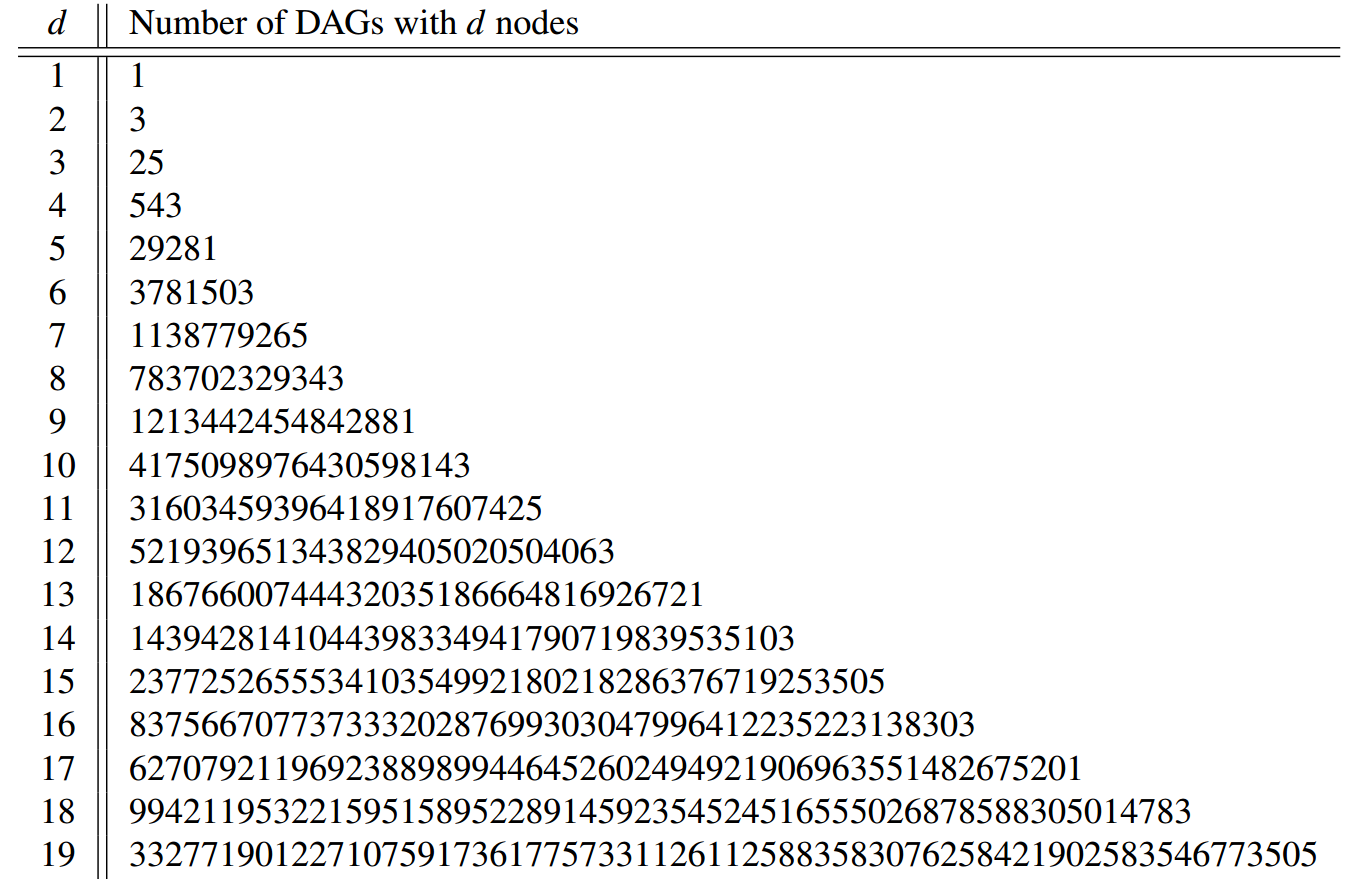
\includegraphics[scale=0.2]{DAGs.png}
\end{frame}

\begin{frame}
	\frametitle{Empirical Experiments}

	Throughout their simulations, they featurize the sample $S = \{(x_i,y_i)\}_{i = 1}^{n}$
	as
	$$\nu(S) = \Big(\mu_{k, m}(P_{S_x}), \mu_{k, m}(P_{S_x}), \mu_{k, m}(P_{S_{xy}})\Big)$$
\pause
\begin{itemize}
\item Motivated by the typical conjecture of existence of asymmetries between the marginal and conditional distributions  of  causally-related  pairs  of  random  variables.

\pause
\item In practice, they set $m= 1000$, and observe no significant improvements when using larger amounts of random features.

\pause
\item Random forest is used for classification.  The  number  of  trees  is chosen from $\{100,250,500,1000,5000\}$ via cross-validation.
\end{itemize}
\textbf{SVM was NOT as good as random foresets}
\end{frame}


\begin{frame}
\frametitle{MPI Cause-Effect Pairs}
Given the small size of the dataset, they decide to use random artificial data in their training set.

\begin{figure}
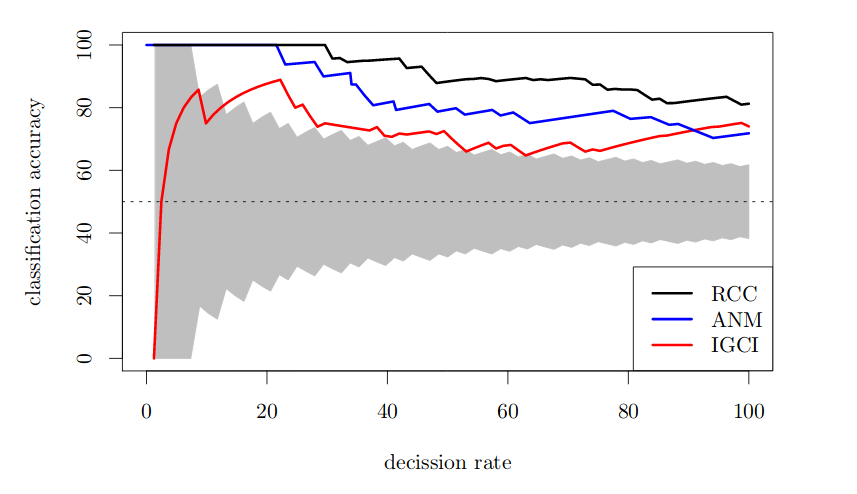
\includegraphics[scale=0.3]{MPI.png}
\end{figure}
\end{frame}




\begin{frame}
\frametitle{Other Expreiments}
\begin{itemize}
	\item Inferring the arrow of time.
	\item ChaLearn’s Challenge Data\\
	199 Training causal samples $S_i$, each drawn from the distribution of $X_i\times Y_i$, and labeled either $X_i \to Y_i$, $Y_i \to X_i$, $Xi\leftarrow Zi\rightarrow Yi$, or "independent".
\end{itemize}
\end{frame}


\begin{frame}
\begin{center}
	\Huge{Thank you!}
\end{center}
\end{frame}
\end{document}

